\documentclass[journal,12pt,twocolumn]{IEEEtran}

\usepackage{setspace}
\usepackage{gensymb}

\singlespacing


\usepackage[cmex10]{amsmath}

\usepackage{amsthm}

\usepackage{mathrsfs}
\usepackage{txfonts}
\usepackage{stfloats}
\usepackage{bm}
\usepackage{cite}
\usepackage{cases}
\usepackage{subfig}

\usepackage{longtable}
\usepackage{multirow}

\usepackage{enumitem}
\usepackage{mathtools}
\usepackage{steinmetz}
\usepackage{tikz}
\usepackage{circuitikz}
\usepackage{verbatim}
\usepackage{tfrupee}
\usepackage[breaklinks=true]{hyperref}
\usepackage{graphicx}
\usepackage{tkz-euclide}

\usetikzlibrary{calc,math}
\usepackage{listings}
    \usepackage{color}                                            %%
    \usepackage{array}                                            %%
    \usepackage{longtable}                                        %%
    \usepackage{calc}                                             %%
    \usepackage{multirow}                                         %%
    \usepackage{hhline}                                           %%
    \usepackage{ifthen}                                           %%
    \usepackage{lscape}     
\usepackage{multicol}
\usepackage{chngcntr}

\DeclareMathOperator*{\Res}{Res}

\renewcommand\thesection{\arabic{section}}
\renewcommand\thesubsection{\thesection.\arabic{subsection}}
\renewcommand\thesubsubsection{\thesubsection.\arabic{subsubsection}}

\renewcommand\thesectiondis{\arabic{section}}
\renewcommand\thesubsectiondis{\thesectiondis.\arabic{subsection}}
\renewcommand\thesubsubsectiondis{\thesubsectiondis.\arabic{subsubsection}}


\hyphenation{op-tical net-works semi-conduc-tor}
\def\inputGnumericTable{}                                 %%

\lstset{
%language=C,
frame=single, 
breaklines=true,
columns=fullflexible
}
\begin{document}


\newtheorem{theorem}{Theorem}[section]
\newtheorem{problem}{Problem}
\newtheorem{proposition}{Proposition}[section]
\newtheorem{lemma}{Lemma}[section]
\newtheorem{corollary}[theorem]{Corollary}
\newtheorem{example}{Example}[section]
\newtheorem{definition}[problem]{Definition}

\newcommand{\BEQA}{\begin{eqnarray}}
\newcommand{\EEQA}{\end{eqnarray}}
\newcommand{\define}{\stackrel{\triangle}{=}}
\bibliographystyle{IEEEtran}
\providecommand{\mbf}{\mathbf}
\providecommand{\pr}[1]{\ensuremath{\Pr\left(#1\right)}}
\providecommand{\qfunc}[1]{\ensuremath{Q\left(#1\right)}}
\providecommand{\sbrak}[1]{\ensuremath{{}\left[#1\right]}}
\providecommand{\lsbrak}[1]{\ensuremath{{}\left[#1\right.}}
\providecommand{\rsbrak}[1]{\ensuremath{{}\left.#1\right]}}
\providecommand{\brak}[1]{\ensuremath{\left(#1\right)}}
\providecommand{\lbrak}[1]{\ensuremath{\left(#1\right.}}
\providecommand{\rbrak}[1]{\ensuremath{\left.#1\right)}}
\providecommand{\cbrak}[1]{\ensuremath{\left\{#1\right\}}}
\providecommand{\lcbrak}[1]{\ensuremath{\left\{#1\right.}}
\providecommand{\rcbrak}[1]{\ensuremath{\left.#1\right\}}}
\theoremstyle{remark}
\newtheorem{rem}{Remark}
\newcommand{\sgn}{\mathop{\mathrm{sgn}}}
\providecommand{\abs}[1]{\left\vert#1\right\vert}
\providecommand{\res}[1]{\Res\displaylimits_{#1}} 
\providecommand{\norm}[1]{\left\lVert#1\right\rVert}
%\providecommand{\norm}[1]{\lVert#1\rVert}
\providecommand{\mtx}[1]{\mathbf{#1}}
\providecommand{\mean}[1]{E\left[ #1 \right]}
\providecommand{\fourier}{\overset{\mathcal{F}}{ \rightleftharpoons}}
%\providecommand{\hilbert}{\overset{\mathcal{H}}{ \rightleftharpoons}}
\providecommand{\system}{\overset{\mathcal{H}}{ \longleftrightarrow}}
	%\newcommand{\solution}[2]{\textbf{Solution:}{#1}}
\newcommand{\solution}{\noindent \textbf{Solution: }}
\newcommand{\cosec}{\,\text{cosec}\,}
\providecommand{\dec}[2]{\ensuremath{\overset{#1}{\underset{#2}{\gtrless}}}}
\newcommand{\myvec}[1]{\ensuremath{\begin{pmatrix}#1\end{pmatrix}}}
\newcommand{\mydet}[1]{\ensuremath{\begin{vmatrix}#1\end{vmatrix}}}
\numberwithin{equation}{subsection}
\makeatletter
\@addtoreset{figure}{problem}
\makeatother
\let\StandardTheFigure\thefigure
\let\vec\mathbf
\renewcommand{\thefigure}{\theproblem}
\def\putbox#1#2#3{\makebox[0in][l]{\makebox[#1][l]{}\raisebox{\baselineskip}[0in][0in]{\raisebox{#2}[0in][0in]{#3}}}}
     \def\rightbox#1{\makebox[0in][r]{#1}}
     \def\centbox#1{\makebox[0in]{#1}}
     \def\topbox#1{\raisebox{-\baselineskip}[0in][0in]{#1}}
     \def\midbox#1{\raisebox{-0.5\baselineskip}[0in][0in]{#1}}
\vspace{3cm}
\title{Assignment 1}
\author{Atla keerthana}
\maketitle
\newpage
\bigskip
\renewcommand{\thefigure}{\theenumi}
\renewcommand{\thetable}{\theenumi}
Download all python codes from 
\begin{lstlisting}
https://github.com/Atlakeerthana/Assignment1/blob/main/Assignment1/assignment1.py
\end{lstlisting}
%
and latex-tikz codes from 
%
\begin{lstlisting}
https://github.com/Atlakeerthana/Assignment1/blob/main/Assignment1/main.tex
\end{lstlisting}
\section{Question No. 2.5}
Draw a $\triangle ABC$ with side $a$ = 7cm, $\angle B = 45^{\degree}$, $\angle A = 105^{\degree}$.
\section{Explanation}
Given,
\begin{align}
\angle A=105\degree,\angle B=45\degree and \text{a}=7
\end{align}
we first need to find $\angle C$:
\\
Finding $\angle C$
\\
In $\triangle ABC$,
\begin{align}
\angle A+\angle B+\angle C = 180^{\degree}
\\
105^{\degree}+45^{\degree}+\angle C = 180^{\degree}
\\
150^{\degree}+\angle C = 180^{\degree}
\\
\angle C = 180^{\degree}-150^{\degree}
\\
\angle C = 30^{\degree}
\end{align}
By law of sines
\begin{align}
\frac{\sin A}{a}=\frac{\sin B}{b}=\frac{\sin C}{c}
\\
\frac{\sin 105^{\degree}}{7}=\frac{\sin 45^{\degree}}{b}=\frac{\sin 30^{\degree}}{c}
\end{align}
we have:
\begin{align}
\frac{\sin 105^{\degree}}{7} &=\frac{\sin 45^{\degree}}{b}
\\
b{\sin 105^{\degree}} &=7{\sin 45^{\degree}}
\\
b &=\frac{7{\sin 45^{\degree}}}{\sin 105^{\degree}}
\\
b &=5.12
\end{align}
similarly,
\begin{align}
\frac{\sin 105^{\degree}}{7} &=\frac{\sin 30^{\degree}}{c}
\\
c{\sin 105^{\degree}} &=7{\sin 30^{\degree}}
\\
c &=\frac{7{\sin 30^{\degree}}}{\sin 105^{\degree}}
\\
c &=3.62
\end{align}
\\
we get values :
\begin{align}
    \implies a &=7;
    \\
    \implies b &=5.12;
    \\
    \implies c &=3.62;
 \end{align}
Now, vertices of given $\triangle ABC$ can be written as,
\begin{align}
\vec{A} &=\myvec{0\\c}=\myvec{0\\3.62}
\\
\vec{B} &=\myvec{0\\0}
\\
\vec{C} &=\myvec{a\\0}=\myvec{7\\0}
\end{align}
\\
Now,$\triangle ABC$ can be plotted using vertices $a$ ,$b$ and $c$
\\
Plot of the angle $\triangle ABC$ :
\numberwithin{figure}{section}
\begin{figure}[!ht]
\centering
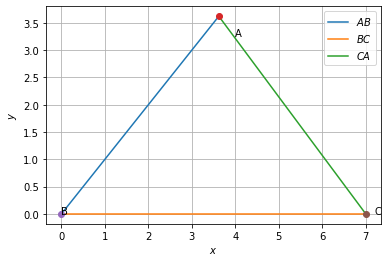
\includegraphics[width=\columnwidth]{figure.png}
\caption{$\triangle ABC$}
\label{fig:$\triangle ABC$}
\end{figure}    
\end{document}